\expandafter\ifx\csname ifdraft\endcsname\relax
   \documentclass[a4j,12pt]{jsreport}
% 数式
\usepackage{amsmath,amsfonts}
\usepackage{bm}

% 画像
\usepackage[dvipdfmx]{graphicx}

% biblatex
\usepackage[style=numeric, sorting=none, maxbibnames=1000]{biblatex}
\addbibresource{graduation_thesis.bib}

%itembox
\usepackage{ascmac}
%breakitemboxのためのpackage
\usepackage{itembkbx}
% \usepackage{tcolorbox} 画像が見えなくなってしまう原因
% \usepackage{framed} 枠

%フォント
\usepackage[ipaex]{pxchfon}

\usepackage[top=35truemm,bottom=30truemm,left=30truemm,right=30truemm]{geometry}
\usepackage{float}
\usepackage{multicol}
\usepackage{multirow}
\usepackage{paralist}
\usepackage{caption}
\usepackage{setspace}
\usepackage{algorithm}
\usepackage{algpseudocode}
\usepackage[dvipdfmx,hidelinks]{hyperref}
\usepackage{pxjahyper}
\usepackage{fancyhdr}
\usepackage{ltablex}
\usepackage{capt-of}
\usepackage{tabularx}
\usepackage{enumitem} % itemizeの行間 これは下になければならない
\usepackage{threeparttable} % 表の脚注


   \setlength{\headheight}{16.5pt}
   \captionsetup{format=hang}
   \begin{document}
   % 上部のヘッダー
\pagestyle{fancy}
\lhead{\rightmark}
\renewcommand{\chaptermark}[1]{\markboth{第\ \thechapter\ 章\ #1}{}}
\fi

\chapter{関連研究}\label{chap:relatedworks}
本章ではまず, \ref{sec:language_model}節で本研究同様, アプリケーションとしてストーリー創作支援システムを構築し, その実践的な活用において有用性と課題が示された研究について紹介し, 次に\ref{sec:story_generation}節で, 物語の生成それ自体を目的とした研究について紹介する.

\section{言語モデルを活用した創作支援システム}\label{sec:language_model}
言語モデルの急速な発展に伴い, これらをストーリークリエーターの創作支援に活用するシステムの研究が進められている.

大曽根ら\cite{Osone21,}は, 日本語小説家に向けた AI との共創による創作支援システム BunCho を提案した. BunCho の操作画面を図\ref{Buncho}に示す.

BunCho の特徴の一つは, 大規模な日本語データセットでファインチューングされた GPT-2 が搭載されていることである. ファインチューニングに用いられた日本語データセットは複数の日本語 web サイトから収集されたブログ記事やニュース記事, 日本語の wikipedia\footnotemark\footnotetext{\url{https://ja.wikipedia.org} (cited 2024-01-27)} およそ 40GB 分のデータと, 創造的な日本語表現を学習させるために使用した, さまざまなカテゴリーにまたがる 11万 以上の日本語 web 小説のデータである. 日本語 web 小説のあらすじからは, 日本人の読者によって不要な表現が削除された. 

もう一つの特徴は, 共創手法の一つとして tabletop role-playing game (TRPG) 型のやり取りが採用されたことである. TRPG とは, 参加者がキャラクターの行動を会話で表現する role-playing game (RPG) である\footnotemark \footnotetext{\url{https://en.wikipedia.org/wiki/Tabletop_role-playing_game} (cited 2024-01-27)}が, このやり取り手法は SNS を通じて BunCho の潜在的ユーザーたちから得たフィードバックをもとに採用された. AI との会話を通じ, キャラクターの行動を表現することでストーリーの創作が行える. 


その他には, 用意されたテンプレートやキーワード, 自由記述, ユーザー自身の SNS 投稿からランダムで取得されたキーワードを用いてタイトルやあらすじの生成を行うことができるシステムが搭載されている. 

16人の様々な執筆経験を持つ作家に BunCho を用いた場合と用いない場合それぞれのあらすじ制作を比較してもらう実験では, 69\% の作家が BunCho を用いたあらすじ制作の方が楽しいと回答し, また 63\% の作家が BunCho を用いたあらすじ制作の方が創造性が拡張されたと回答した. 作家から得たポジティブな感想には, 自分では思いつかないストーリーを作ることができたということや初心者の作家は BunCho を使うことであらすじの制作が簡単になるのではないかといった感想があり, ネガティブな感想には, BunCho が生成するストーリーに一貫性がないことやインターフェースがわかりにくという感想があった. 32 人の読者に, 制作されたあらすじを BunCho による支援の有無は知らせず次の 5つの指標, 創造性, 面白さ, 理解可能性, 文法的正確性, 文章の一貫性で評価してもらう実験では, 69\% の作家の作品において, 5つの指標のうち少なくとも一つの指標で BunCho を用いたものが作家自身で書いたものに比べ改善される可能性が示された. しかしながらいずれも高い優位性を誇るという結果を得ることには至らなかった.

本研究では, 直感的な操作を提供するインターフェースにより操作の容易性を向上するよう努め, 現段階における最先端モデル GPT-4 を用いることにより, BunCho における一貫性の欠如を改善することを目指した.

\begin{figure}[H]
   \centering
   \includegraphics[width=12cm]{pict/03/Buncho.png}
   \caption[BunChoの操作画面]{BunCho の操作画面 \protect\footnotemark }
   \label{Buncho}
\end{figure}
\vspace{-15pt}
\footnotetext{\cite{Osone21}より引用. \url{https://bun-cho.work/} (cited 2024-01-27)}  

Yuanら\cite{yuan22}は, 大規模言語モデル LaMDA\cite{thoppilan22} を活用したストーリー制作が行えるテキストエディタ Wordcraft を提案した. LaMDA は, Google が開発した 1370億個のパラメータを持つ, Transformer のデコーダ部分のみを用いた左から右へ単方向に予測を行う大規模言語モデルである. LaMDA は以下に示した対話例のように, 会話のシーケンスから次の返答を予測する. 

\begin{quote}
   \textbf{prompt:} A: Can you help me write a short story about aliens? \\
   B: Sure. I’m happy to help. \\
   A: What is a good name for my story? \\
   \textbf{LaMDA:} B: It depends on the story. If it’s a dark story, call it The Dark Side.\footnotemark
\end{quote}
\footnotetext{\cite{yuan22}より引用.}

Wordcraft における操作画面の例を図\ref{Wordcraft}に示す. Wordcraft では主に5つの機能が搭載されており, Infilling と名付けられた機能では, ユーザー自身で書いたテキストの一部を選択することで, その代替案を生成させることができ, Continuation と名付けられた機能では, ユーザー自身で書いたテキスト内に置くカーソル位置に合わせ, その箇所に合う文章を生成させ挿入することができる. Wordcraft では, プロンプトに関する工夫も施されている. 5つの機能はそれぞれ事前に用意されたプロンプトで動作させられるが, ユーザー自身の言葉でプロンプトをカスタムし動作させることもできる. また, ユーザー自身の意図がよく反映させられるように, プロンプト自体を生成させることができる Meta-Prompting という機能も備えている.

Wordcraft を評価する実験として3つの条件が比較された. 一つは Wordcraft の全ての機能がつかえる条件. もう一つは機能を, 従来のシステムにも搭載されている機能, 文章の続きを生成させることができる機能のみに限定した条件. 最後の一つは, LaMDA とチャット形式のやり取りが行えるウィンドウを横に, テキストエディタ自体はプレーンなものにする条件である. 参加者は, 参加者ごとにそれぞれの条件で物語を作成するよう依頼され, 物語の作成後 8 つの質問に対し5段階のリッカート尺度で Wordcraft を評価するよう求められた. その結果, 全ての機能が使える条件で物語を作成した参加者が, 他の条件で物語を作成した参加者よりも, 優位に Wordcraft を役立つものと回答した. しかしながら, AIのストーリーに対する認識の欠如や生成物の一貫性が不足しているという評価も受けた.  

本研究では, 物語構造分析をLLMの制御に活用することで, 一貫性を保つ物語の生成に取り組んだ.

\begin{figure}
   \centering
   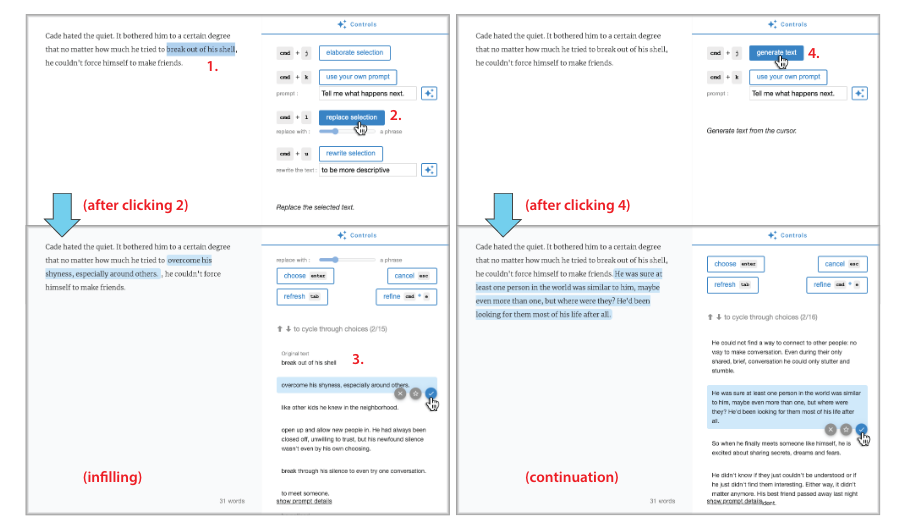
\includegraphics[width=12cm]{pict/03/Wordcraft.png}
   \caption[Wordcraft の操作画面]{Wordcraft の操作画面 \protect\footnotemark}
   \label{Wordcraft}
\end{figure}


Mirowskiら\cite{mirowski23}は, ストーリー創作において, 長距離意味的な一貫性を欠く言語モデルの課題に対処するため, 言語モデルの段階的な適用を通じて共創の有用性を高めるDramatronと呼ばれるシステムを提案した. このシステムは, 映画や演劇の脚本を, 言語モデルを介した段階的な創作プロセスを通じて構築することを目的としたシステムである.
\footnotetext{\cite{yuan22}より引用. \url{https://www.youtube.com/watch?v=HthbABWE-xw} (cited 2024-01-27)} 

このシステムで用いられている言語モデルは, Chinchilla\cite{hoffmann22}と呼ばれる大規模言語モデルで,  1.4Tトークンで学習した700億個のパラメータを持つモデルである. その特徴は, スケーリング則に基づきパラメータ数と学習データ量のバランスが考慮されたことであり, 比較的小さなパラメータ数でGPT-3の性能を上回っている.

Dramatronにおける段階的な脚本制作を図\ref{Dramatron}に示す. Log line と呼ばれるストーリーの要約文から作成し, そこからタイトルとキャラクターを作成, その後作成したキャラクターをプロンプトに用い, プロットとして一連の要約されたシーン展開を作成する. その後, それぞれのシーンの詳細な設定を含むロケーションを作成したのち, これまで作成された全てを組み合わせてキャラクター同士の会話, セリフを作成する. この各段階においてユーザーからのフィードバックを都度反映させることができ, 物語の一貫性を保つ.

15人の劇場や映画業界の専門家による利用を通じた評価では, Dramatron の利用は楽しく, 驚きのあるものであったという評価や, 制作された作品の一貫性が良いという評価を得た. 一方で, 制作された作品が自分自身のものであるという感覚が低いという評価を得た.

\begin{figure}[H]
   \centering
   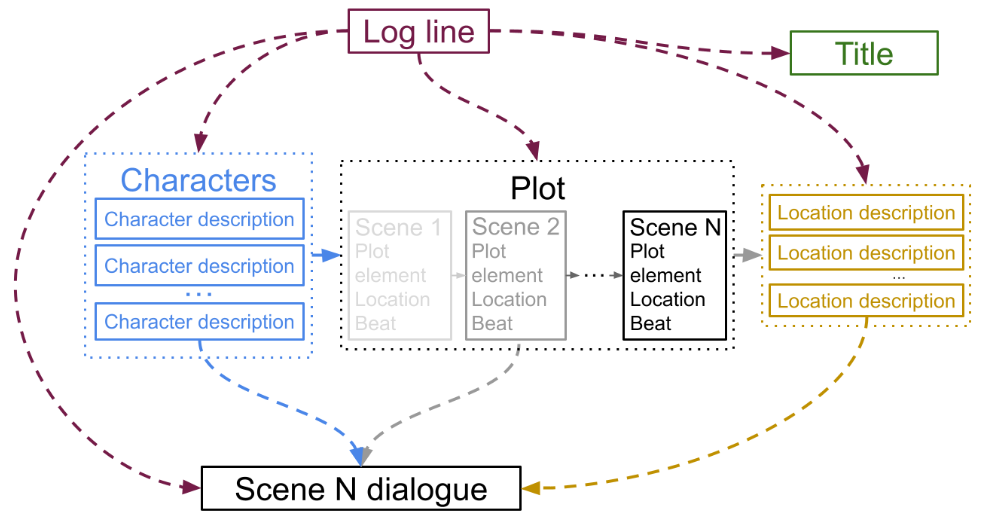
\includegraphics[width=10cm]{pict/03/Dramatron.png}
   \caption[Dramatron における段階的な脚本制作]{Dramatron における段階的な脚本制作 \protect\footnotemark}
   \label{Dramatron}
\end{figure}
\footnotetext{\cite{mirowski23}より引用.}
%利用した作家からは, AIとの共創体験が楽しいものであったという評価を受けた. 一方で, 生成物の正確さや一貫性という観点では, 人の手で書かれたものよりも有意に低い評価を受けた.

 %AI との対話によって文章を改変していくことができるシステムであるが, AI の返答がうまく文脈を認識していないと感じられる課題が生じている. 

 \section{物語生成}\label{sec:story_generation}

日笠ら\cite{higasa23}は, 物語の生成に関する手法を「ニューラルアプローチ」と「シンボリックアプローチ」の2つに分類している. 「ニューラルアプローチ」とは, 物語生成においてニューラルネットワークを用いた手法であり, 上記に挙げたシステムにおいて行われる言語モデルの物語生成は, ニューラルアプローチの枠組みに含まれるものと考えられる. 「シンボリックアプローチ」とは, 物語を記号として扱いその順序などに応じて物語を生成する手法である. この手法の一つとしてLiらが提案した手法を挙げることができる.

Liら\cite{Li13}はクラウドソーシングの活用により, 物語のドメインモデルを自動的に学習して未知のドメインに対し物語を生成する手法を提案した. 具体的にはまず, クラウドソーシングを用いて特定のトピックに関する多数の物語を収集する. それらをもとにプロットグラフと呼ばれるドメインモデルを自動的に構築し, プロットグラフを利用することで未知のトピックに関する物語の生成を行う. プロットグラフとは, 物語の中で起こる出来事をノードとし, それら出来事の前後関係をエッジで表現したものである. プロットグラフの例を図\ref{Plotgraph}に示す. この手法は, ドメインモデルを利用する従来の物語生成手法がドメインモデルの作成を人手で行う必要があったのに対し, 自動でドメインモデルを作成することができスケーラブルであるという点で優れている. また, クラウドソーシングの利用は, 収集される物語の多様性を増加させる利点もある. 実験により, この手法で生成された物語は, プロではない一般の方が作成した物語と同程度の品質をもつとして評価された. 

\begin{figure}[H]
   \centering
   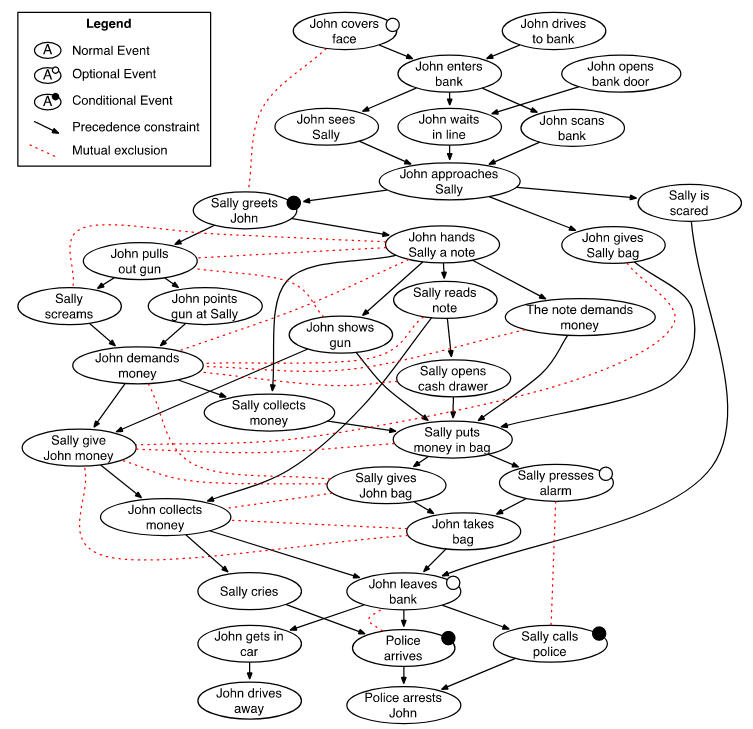
\includegraphics[width=10cm]{pict/03/Plotgraph.png}
   \caption[プロットグラフの例]{プロットグラフの例 \protect\footnotemark}
   \label{Plotgraph}
\end{figure}
\footnotetext{\cite{Li13}より引用.}

日笠ら\cite{higasa23}は, 上記の2分類を混合し物語生成を行う手法を提案した. 物語構造というシンボリックな情報を活用し, GPT-3を制御することで生成したプロットユニットを, 意味的類似度で繋ぎ合わせプロットの自動生成を行なうというものである. ここでいうプロットとは, 物語の大きな流れを示す文章のことであり, プロットユニットとは, プロットを展開ごとに分割した要素のことを表す. この手法における概略を図\ref{} に示す. この研究により, プロット生成における物語構造の有用性が示唆された. しかしながら, このシステムはクリエーターが直接操作できず, クリエーターの意思を反映することができないうえ, 異なるドメインのプロットユニットを繋ぎ合わせることで, 一貫性のないプロットが生成されるという課題があった.

\begin{figure}[H]
   \centering
   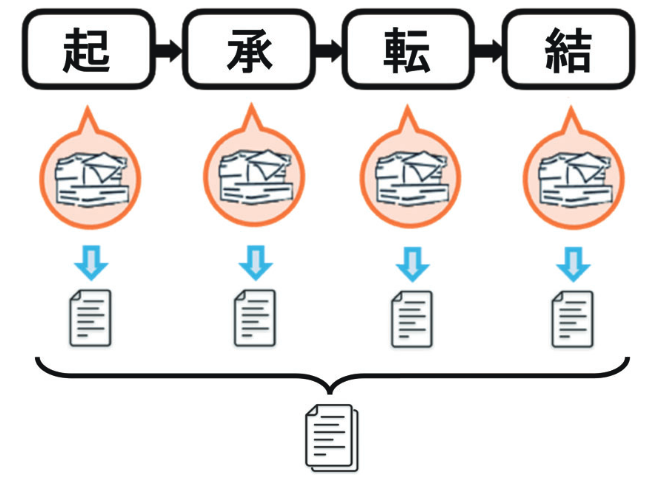
\includegraphics[width=6cm]{pict/03/higasa.png}
   \caption[日笠らの研究で用いられた物語生成手法の概略図]{日笠らの研究で用いられた物語生成手法の概略図 \protect\footnotemark}
   \label{Plot}
\end{figure}
\footnotetext{\cite{higasa23}より引用.}

本研究では, GPT-4の性能の高さを利用し, 物語構造の活用をプロット自体の生成に適応する手法を提案する.


\expandafter\ifx\csname ifdraft\endcsname\relax
   \fancyhead[LO]{}
   \printbibliography[title=参考文献]
   \end{document}
   \fancyhead[LO]{\rightmark}
\fi
